%%%%%% CMB-S4 Simulations and Data Analysis Chapter, Implementation Section  %%%%%%%%%%%%%%%%
 
\section{The Production Data Pipeline}

With real data in hand, the production data pipeline (Figure \ref{fig_prod}) will include data analysis, time-domain simulation for uncertainty quantification, and feedback loops to improve both the mission model and the sky simulation. Time domain data are extensively used to refine our model of the mission; for the instrument model this can include such steps as determining beam profiles and estimating noise properties (including cross-correlations); for the observation model, it includes reconstructing the detector pointing and polarization orientation from telescope sensor data, and incorporating atmosphere records in the data-flagging. The foreground component maps, observed spectra, and parameters of cosmology and fundamental physics are used to refine our sky model. In both cases the feedback loops both improve the consistency of the simulations with the data and enable us to refine the validation and verification of the analysis methods themselves.

\begin{figure}[htbp]
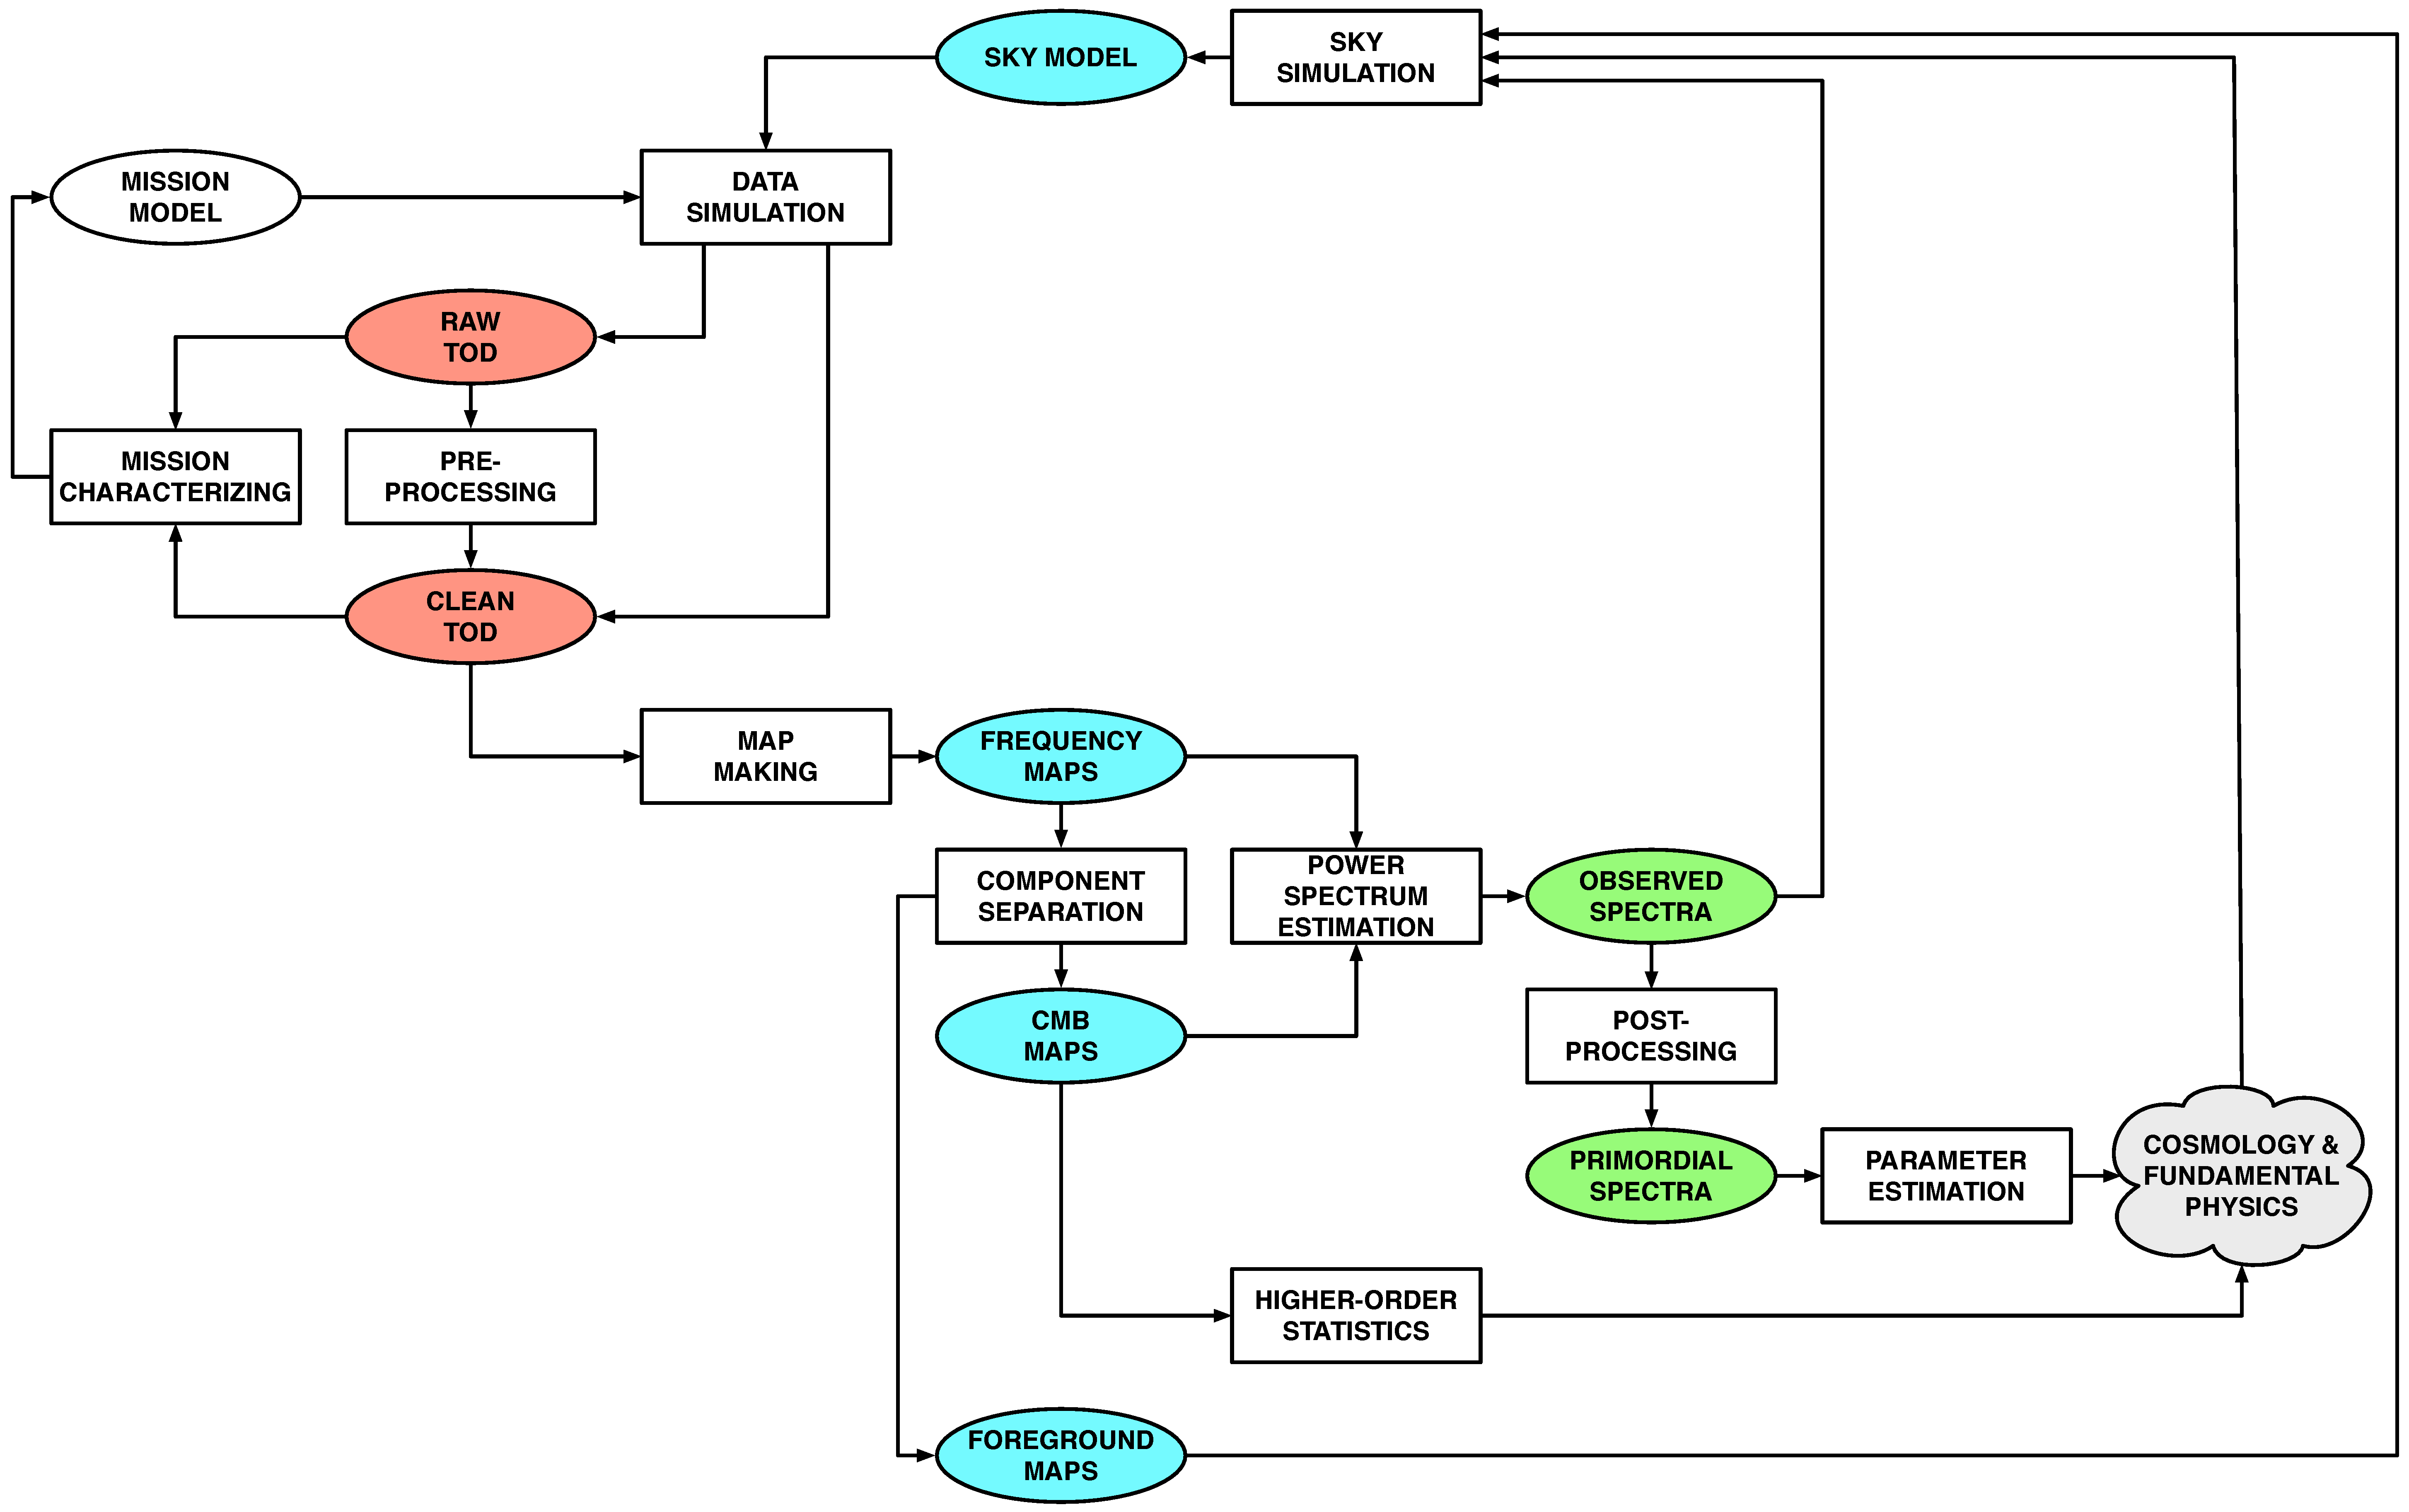
\includegraphics[width=1.0\textwidth]{Analysis/production_figure}\\
\caption{The production data pipeline, including data analysis, simulation, and feedback.}
\label{fig_prod}
\end{figure}

\subsection{Implementation Issues}

The quest for ever-fainter signals in the CMB drives us to gather ever-larger time-ordered data (TOD) sets to obtain the necessary signal-to-noise to uncover them. As Figure \ref{fig_cmb_hpc_scaling} shows, the volumes of ground-based, balloon-borne and satellite CMB data sets have exhibited exponential growth over the last two decades, and are anticipated to do so again over the coming two. Moreover, for suborbital experiments the exponent exactly matches that of Moore's Law for the growth of computing capability, where we use as a proxy here the peak performance of the flagship high performance computing (HPC) system at the DOE's National Energy Research Scientific Computing (NERSC) Center at any epoch (reflecting the widespread use of NERSC for CMB data analyses over the last 20 years). 

\begin{figure}[htbp]
\centering
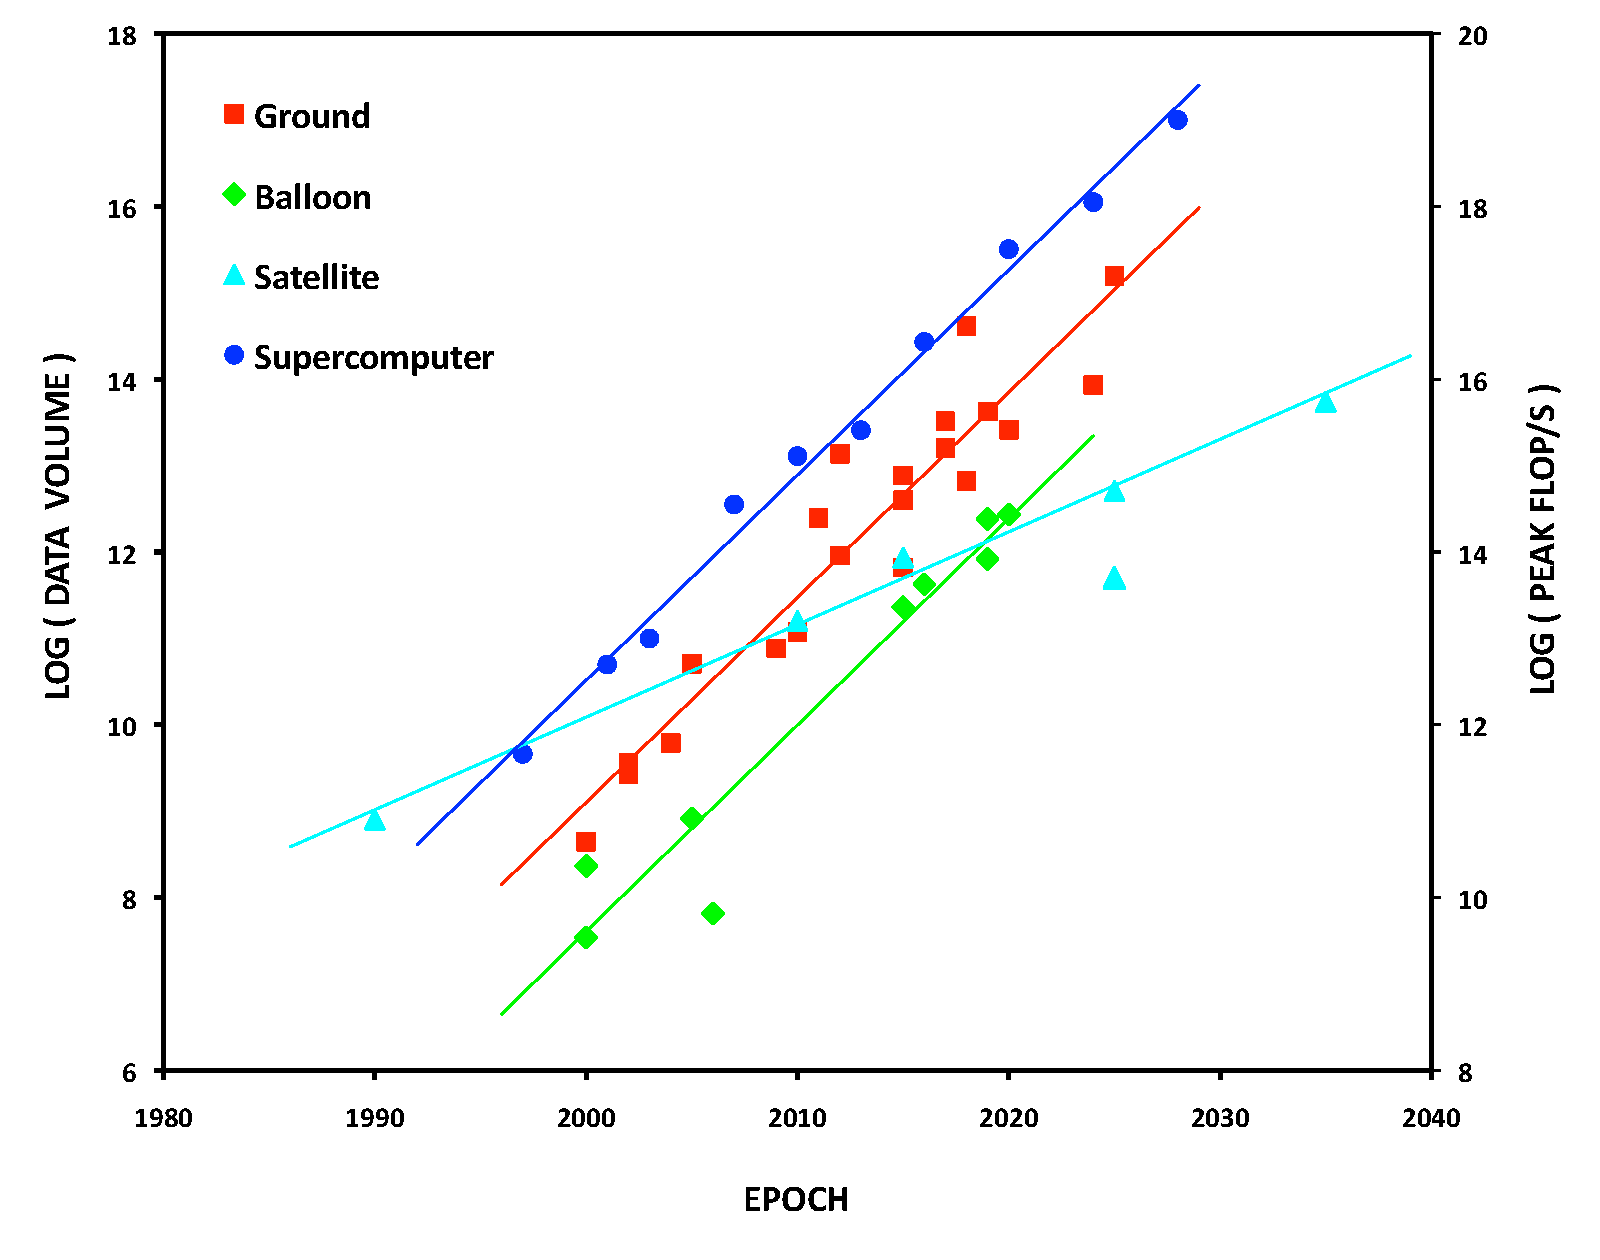
\includegraphics[width=0.75\textwidth]{Analysis/cmb_hpc_scaling}
\caption{Exponential growth of CMB time-ordered data volume and HPC capability: 1990 -- 2030.}
\label{fig_cmb_hpc_scaling}
\end{figure}

As noted above, in the absence of a full data covariance matrix we rely on Monte Carlo methods for uncertainty quantification and debiasing, and achieving the desired percent-level statistical uncertainty requires us to simulate and reduce $10^4$ realizations of the data. This implies that all TOD-processing steps (in simulation or analysis) must employ algorithms that scale no worse than linearly in the number of samples, and that these algorithms must {\em collectively} be implemented efficiently on the largest high performance computing (HPC) platforms available to us. 

The most massive Monte Carlo sets generated to date have been the Full Focal Plane (FFP) sets in support of the analysis of the \planck\ satellite data \cite{Ade:2015via}, with FFP8 comprising $10^4$ realizations of the mission reduced to O($10^6$) maps. Key to achieving this scale has been an aggressive optimization of the software stack, coupled with system-specific tuning over 6 generations of NERSC supercomputer. In particular wherever possible TOD input/output (IO) is removed from the pipeline so that, for example, instead of pre-computing the TOD and then pre-processing/mapping it, each realization is generated on demand and passed to the analysis pipeline in memory. While this necessitates the re-simulation of a realization should further analysis be required, it is still very substantially faster than writing it to disk and reading it back in. Similarly, inter-process communication is optimized by using a hybridized MPI/OpenMP implementation that employs explicit message passsing for inter-node, and threading for intra-node, communication.

The critical challenge for CMB-S4 will be to develop these capabilities for a dataset 1000x the size of \planck's and 100x the size of those from existing S2 ground-based experiments. This scale of computing will require substantial development effort from the CMB community, but is still much smaller than some existing experiments (e.g. ATLAS, CMS) and, with appropriate tooling, should be possible on existing or forthcoming computing facilities. The S3 experimental efforts are currently exploring a number of computational tools to reach the required level, including investigating use of the US grid where feasible and code optimization for the upcoming generations of energy-constrained HPC architectures, with their increased heterogeneity and deeper memory hierarchies and based, in the short term, on either graphical programming unit (GPU) or many integrated core (MIC) technologies.


